% arara: xelatex
% arara: xelatex
% arara: xelatex

% options:
% thesis=B bachelor's thesis
% thesis=M master's thesis
% czech thesis in Czech language
% english thesis in English language
% hidelinks remove colour boxes around hyperlinks

\documentclass[thesis=M,english]{prefs/FITthesis}[2019/03/06]

% \usepackage{subfig} %subfigures
% \usepackage{amsmath} %advanced maths
% \usepackage{amssymb} %additional math symbols

\usepackage[utf8]{inputenc}

\usepackage{graphicx} %graphics files inclusion
% \usepackage{amsmath} %advanced maths
% \usepackage{amssymb} %additional math symbols

\usepackage{dirtree} %directory tree visualisation
\usepackage{subfig} %image side by side
\usepackage{todonotes} %todo
\usepackage{url}
\usepackage{textcomp} %degree symbol
\usepackage{color, colortbl} %color, table color
\usepackage{enumitem} %lists
\usepackage{float} %for H option in figures
\usepackage{array} %table aligment       
\usepackage{amsmath} %cases
\usepackage{amssymb}
\usepackage{svg} %svg
\usepackage{scrextend}
\usepackage{multirow}
\addtokomafont{labelinglabel}{\sffamily}

\definecolor{LightCyan}{rgb}{0.88,1,1}
\definecolor{Blue}{rgb}{0.30980, 0.50588, 0.73725}
\definecolor{White}{rgb}{1, 1, 1}

% list of acronyms
\usepackage[acronym,nonumberlist,toc,nopostdot,numberedsection=autolabel,nomain]{glossaries}
\makeglossaries
\newcommand{\tg}{\mathop{\mathrm{tg}}} %cesky tangens
\newcommand{\cotg}{\mathop{\mathrm{cotg}}} %cesky cotangens

% % % % % % % % % % % % % % % % % % % % % % % % % % % % % % % % % % % 
% % % % % % % % % % % % % % % % % % % % % % % % % % % % % % % % % % % 
\department{Department of Applied Mathematics}
\title{Vehicle Routing Problem with Time Windows solved via Machine Learning and Optimization Heuristics}
\authorGN{Adam} %author's given name/names
\authorFN{Zvada} %author's surname
\authorWithDegrees{Bc. Adam Zvada} %author's name with academic degrees
\author{Adam Zvada} %author's name without academic degrees
\supervisor{doc. Ing. Pavel Kordík, Ph.D.}
\acknowledgements{TODO}
\abstractCS{TODO}
\abstractEN{TODO}
\placeForDeclarationOfAuthenticity{Prague} %where you have signed the declaration
\keywordsCS{TODO\newpage}
\keywordsEN{TODO}
\declarationOfAuthenticityOption{5} %select as appropriate, according to the desired license

\newacronym{ai}{AI}{artificial intelligence}
\newacronym{vrp}{VRP}{vehicle routing problem}
\newacronym{cvrp}{CVRP}{capacitated vehicle routing problem}
\newacronym{vrptw}{VRPTW}{vehicle routing problem with time windows}
\newacronym{tsp}{TSP}{traveling salesman problem}
\newacronym{ml}{ML}{machine learning}
\newacronym{pdp}{PDP}{Pick and Deliver}
\newacronym{vrppd}{VRPPD}{vehicle routing problem with pick and deliver}
\newacronym{rl}{RL}{reinforcement learning}

\newacronym{ctu}{CTU}{Czech Technical University}
\newacronym{cpu}{CPU}{central processing unit}
\newacronym{cv}{CV}{computer vision}
\newacronym{dex}{DEX}{Deep EXpectation}
\newacronym{dl}{DL}{deep learning}
\newacronym{dlt}{DLT}{Direct Linear Transform}
\newacronym{dsae}{DSAE}{deep sparse autoencoders}
\newacronym{fast r-cnn}{Fast R-CNN}{fast region-based convolutional network}
\newacronym{faster r-cnn}{Faster R-CNN}{faster region-based convolutional network}
\newacronym{fce}{FCE}{Faculty of Civil Engineering}
\newacronym{fit}{FIT}{Faculty of Information Technology}
\newacronym{fn}{FN}{false negatives}
\newacronym{fp}{FP}{false positives}
\newacronym{fps}{FPS}{frames per second}
\newacronym{gige}{GigE}{Gigabit Ethernet}
\newacronym{gpu}{GPU}{graphics processing unit}
\newacronym{hog}{HOG}{histogram of oriented gradients}
\newacronym{hsv}{HSV}{hue-saturation-value}
\newacronym{idsw}{IDSW}{identity switches}
\newacronym{improlab}{ImproLab}{Image Processing Laboratory}
\newacronym{iou}{IoU}{intersection over union}
\newacronym{lbp}{LBP}{local binary pattern}
\newacronym{lstm}{LSTM}{long short-term memory}
\newacronym{mae}{MAE}{mean absolute error}
\newacronym{ml}{ML}{machine learning}
\newacronym{mlp}{MLP}{multi layer perceptron}
\newacronym{mot}{MOT}{multiple object tracking}
\newacronym{mota}{MOTA}{multiple object tracking accuracy}
\newacronym{motp}{MOTP}{multiple object tracking precision}
\newacronym{mots}{MOTS}{multiple object tracking and segmentation}
\newacronym{mp}{MP}{megapixel}
\newacronym{mtmct}{MTMCT}{multi-target multi-camera tracking}
\newacronym{nms}{NMS}{non-maximum suppression}
\newacronym{nn}{NN}{neural network}
\newacronym{pca}{PCA}{principal component analysis}
\newacronym{r-cnn}{R-CNN}{region-based convolutional network}
\newacronym{reid}{ReID}{re-identification}
\newacronym{rgb}{RGB}{red-green-blue}
\newacronym{roi}{RoI}{region of interest}
\newacronym{rmse}{RMSE}{root-mean-square error}
\newacronym{rnn}{RNN}{recurrent neural network}
\newacronym{rpn}{RPN}{region proposal network}
\newacronym{sdk}{SDK}{software development kit}
\newacronym{sift}{SIFT}{Scale-invariant feature transform}
\newacronym{sort}{SORT}{simple online and real-time tracking}
\newacronym{ssd}{SSD}{single-shot detector}
\newacronym{ssr}{SSR-Net}{Soft Stagewise Regression Network}
\newacronym{surf}{SURF}{Speeded-Up Robust Features}
\newacronym{spp}{SPP}{spatial pyramid pooling}
\newacronym{svm}{SVM}{support vector machine}
\newacronym{yolo}{YOLO}{you only look once}


\begin{document}
    \begin{introduction}
    The \gls{vrp} is one of the most extensively studied combinatorial problems. It is easy to define but very difficult to solve\cite{time-complexity-vrp}. The reason \gls{vrp} is attracting many researchers is the fact that finding a near-optimal solution in a reasonable time would have a great impact on many industries, especially in the domain of transportation and logistics. 
    
    \begin{figure}[ht]
        \centering
        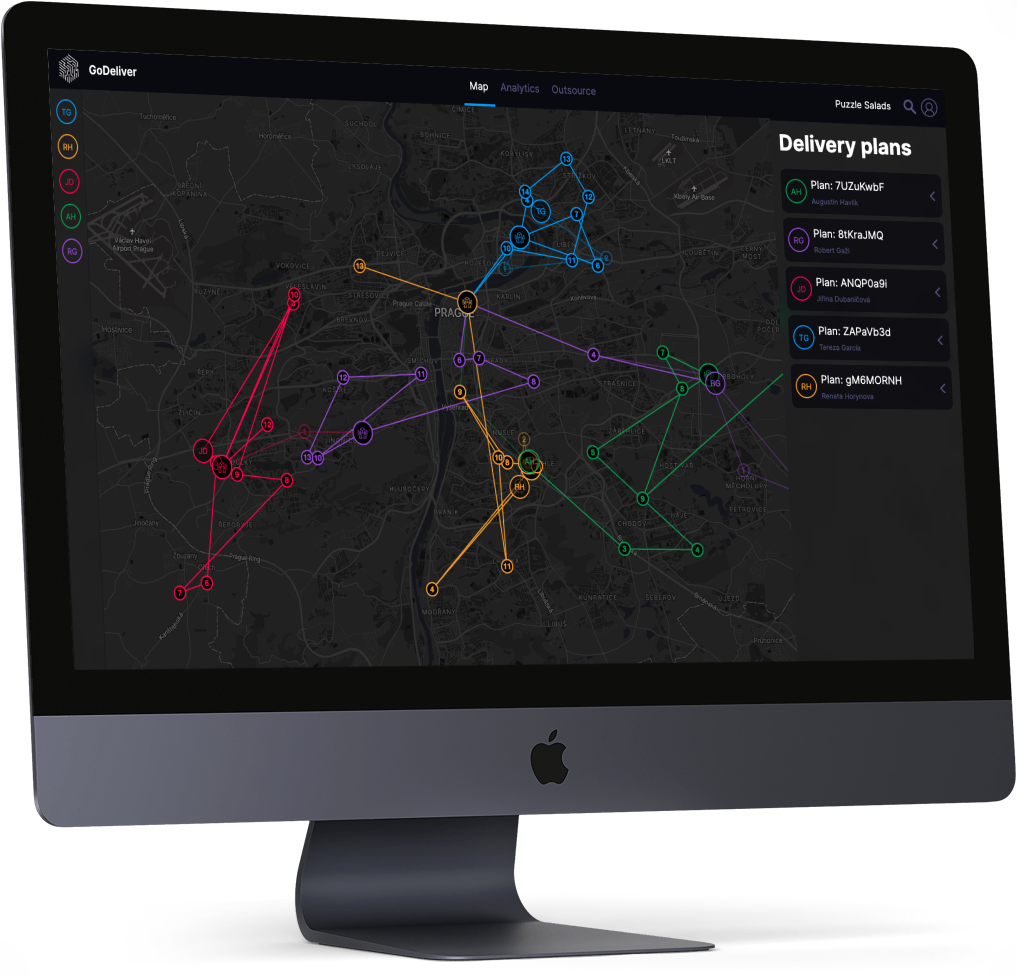
\includegraphics[width=0.5\textwidth]{resources/intro/godeliver-dashboard.png}
        \caption{GoDeliver dashboard visualizing solution for an instance of vehicle routing problem with time windows.}
        \label{fig:godeliver_dashboard}
    \end{figure}
    
    \section{Motivation}
    The paradigm shift in logistics business models towards instant gratification of customers are pushing the planning systems to be flexible and dynamic. The environment is constantly changing and planning systems have to update or entirely replan the instance in a short amount of time but maintaining the best delivery efficiency. Having a powerful planning system results in a dramatic reduction of delivery expanses.
    
    \section{Challenges}
    In the real world, the general VRP problem is not enough to solve the business-related problems. \gls{vrp} has multiple variants adding various constraints such as capacity, demand or time windows for given set of customers. The \gls{vrptw} is main focus of this thesis and we will be looking at some novel approaches how to solve it with \gls{ai}.
    
    \section{Assumptions} 
    We expect that leveraging \gls{ai} or \gls{ml} techniques to solve \gls{vrp} would lead in a drastic reduction of computational time for solving given instance of \gls{vrp}. Moreover, the time complexity would not be exponentially increasing with the problem size. The trade-off lays in the required time to allow \gls{ai} to train and learn how to solve the problem of vehicle routing.
    
    \section{Thesis structure}
    The rest of this thesis is organized as follows:
    \begin{itemize}
        \item Chapter \ref{introduction_vrp} presents a formal introduction to Vehicle Routing Problem.
        \item Chapter \ref{theoretical_background} provides an advanced theoretical background.
        \item Chapter \ref{vrptw-optimization} describes solutions of \gls{vrptw} for optimization heuristics.
        \item Chapter \ref{system} describes how a delivery planning system works.
        \item Chapter \ref{vrptw-ai} describes the proposed method for solving \gls{vrptw} via deep learning.
        \item Chapter \ref{evaluation} evaluates and benchmarks the proposed deep learning model.
    \end{itemize}
\end{introduction}
    \chapter{Introduction to Vehicle Routing Problem}\label{introduction_vrp}

    The problem objective of \gls{vrp} is simply finding the shortest route for multiple vehicles to serve all the given set of customers. The shortest route can be differently interpreted based on your minimalization criteria, e.g, traveled distance, time, or a combination of both. It was first proposed by Dantzig and Ramser \cite{truck-dispatching-problem} in 1959, and since then researchers are coming up with different approaches how to solve the problem. 

    \section{Vehicle Routing Problem Definition}
    
    The general \gls{vrp} can be defined as a problem in a complete graph $G=(V,E)$ of finding the optimal permutation $\pi_l = (\pi_0, \cdots, \pi_m)$ of nodes $V$ all starting from a node $v_0$ for given number of paths $k$ which results in minimal traversal cost where $\forall v \in (V \setminus v_0)$ are visited only once. \gls{vrp} is generalization of \gls{tsp} which only has one path.
    
    \begin{figure}[ht]
        \centering
        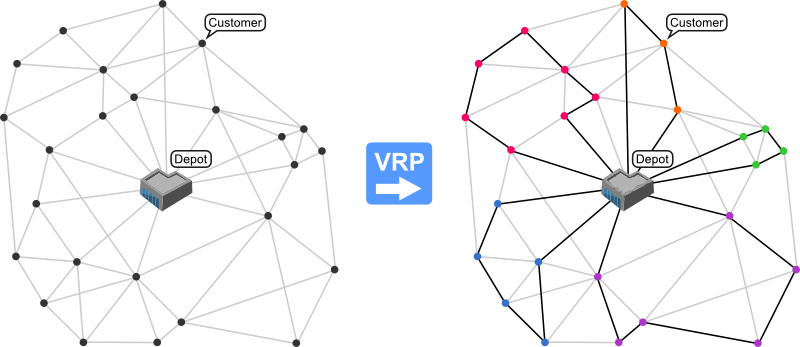
\includegraphics[width=0.75\textwidth]{resources/intro/vrp-graph.png}
        \caption{Intuitive view of \gls{vrp} instance on left and proposed solution for 5 vehicles on the right \cite{vrp-malaga}}
        \label{fig:vrp-graph}
    \end{figure}
    
    \gls{vrp}s are classified as NP-Hard problems which was proved by Lenstra and Kan \cite{time-complexity-vrp}. It means that in the worst case, adding new nodes, i.e., customers results in an exponential increase of computational complexity.
    
    \subsection{VRP Notation}
    Let's introduce our used notation and its real-world interpretation.
    \begin{itemize}
        \item $G=(V,E)$ is a complete undirected graph
        \begin{itemize}
            \item Network of routes
        \end{itemize}
        \item $v_0$ is the initial node
        \begin{itemize}
            \item A depot
        \end{itemize}
        \item $V^{\prime} = (v_1, \cdots, v_n)$ nodes expect the initial node
        \begin{itemize}
            \item Geographically scattered location of customers
        \end{itemize}
        \item $E = \{(v_i, v_j)| v_i, v_j \in V, i \neq j\}$ with associated weight as a cost $c: E \to \mathbb{N}^+$
        \begin{itemize}
            \item A single route between two locations with associated cost, e.g., distance.
        \end{itemize}
        \item $C$ is a matrix of edge weights indexed by nodes. $c_i_j$ where $i,j \in V$
        \begin{itemize}
            \item Matrix of costs between customers
        \end{itemize}
        \item $R_i \subset V$ is a path that starts and ends at $v_0$. $(r_0 = v_0 \land r_{|R_i|} = v_0)$
        \begin{itemize}
            \item Route visit a subset of customers starting and ending at the depot, it can be referred to it as a delivery plan.
        \end{itemize}
        \item $k$ number of paths
        \begin{itemize}
            \item Number of vehicles
        \end{itemize}
        \item $R = R_1, \cdots, R_k$ is a set of paths
        \begin{itemize}
            \item All routes (delivery plans) for a given instance of \gls{vrp}.
        \end{itemize}
        \item $\pi = (\pi_1, \cdots, \pi_k)$ solution for a given instance of \gls{vrp}.
        \begin{itemize}
            \item Customer locations in visiting order for multiple vehicles.
        \end{itemize}
    \end{itemize}
    
    \textbf{Feasibility of \gls{vrp} solution} for \gls{vrp} of routes $R$ is feasible only if each node $V_1$ is visited exactly once.
    
    \textbf{The cost of route $R_i$} which we aim to minimize is the sum of its weights (costs). If we operate in Euclidean space, then it is L2 norm of route locations.
    \begin{equation}
        C(R_i) := \sum_{k = 0}^{|R_i|} c_{r_k}_{r_k+1}
    \end{equation}
    
    \textbf{The cost of \gls{vrp} solution} is the sum of route costs.
    \begin{equation}
        C(R) := \sum_{i = 1}^{|R|} C(R_i)
    \end{equation}
    
\section{Vehicle Routing Flavors}
Our modern world heavily relies on complex logistics networks. It requires to synchronize multimodal planning to ship your goods from one side of the world to your doorstep. In order to achieve this, multiple variants and flavours of \gls{vrp} had to be studied and implemented in the real world use cases. It goes from ordinary variants like measuring the capacity of cars to a more niche problem like eVRP where vehicles are required to make stops to recharge.

All the flavours of \gls{vrp} can be mutually combined, which is usually the main area of research.

    \begin{figure}[ht]
        \centering
        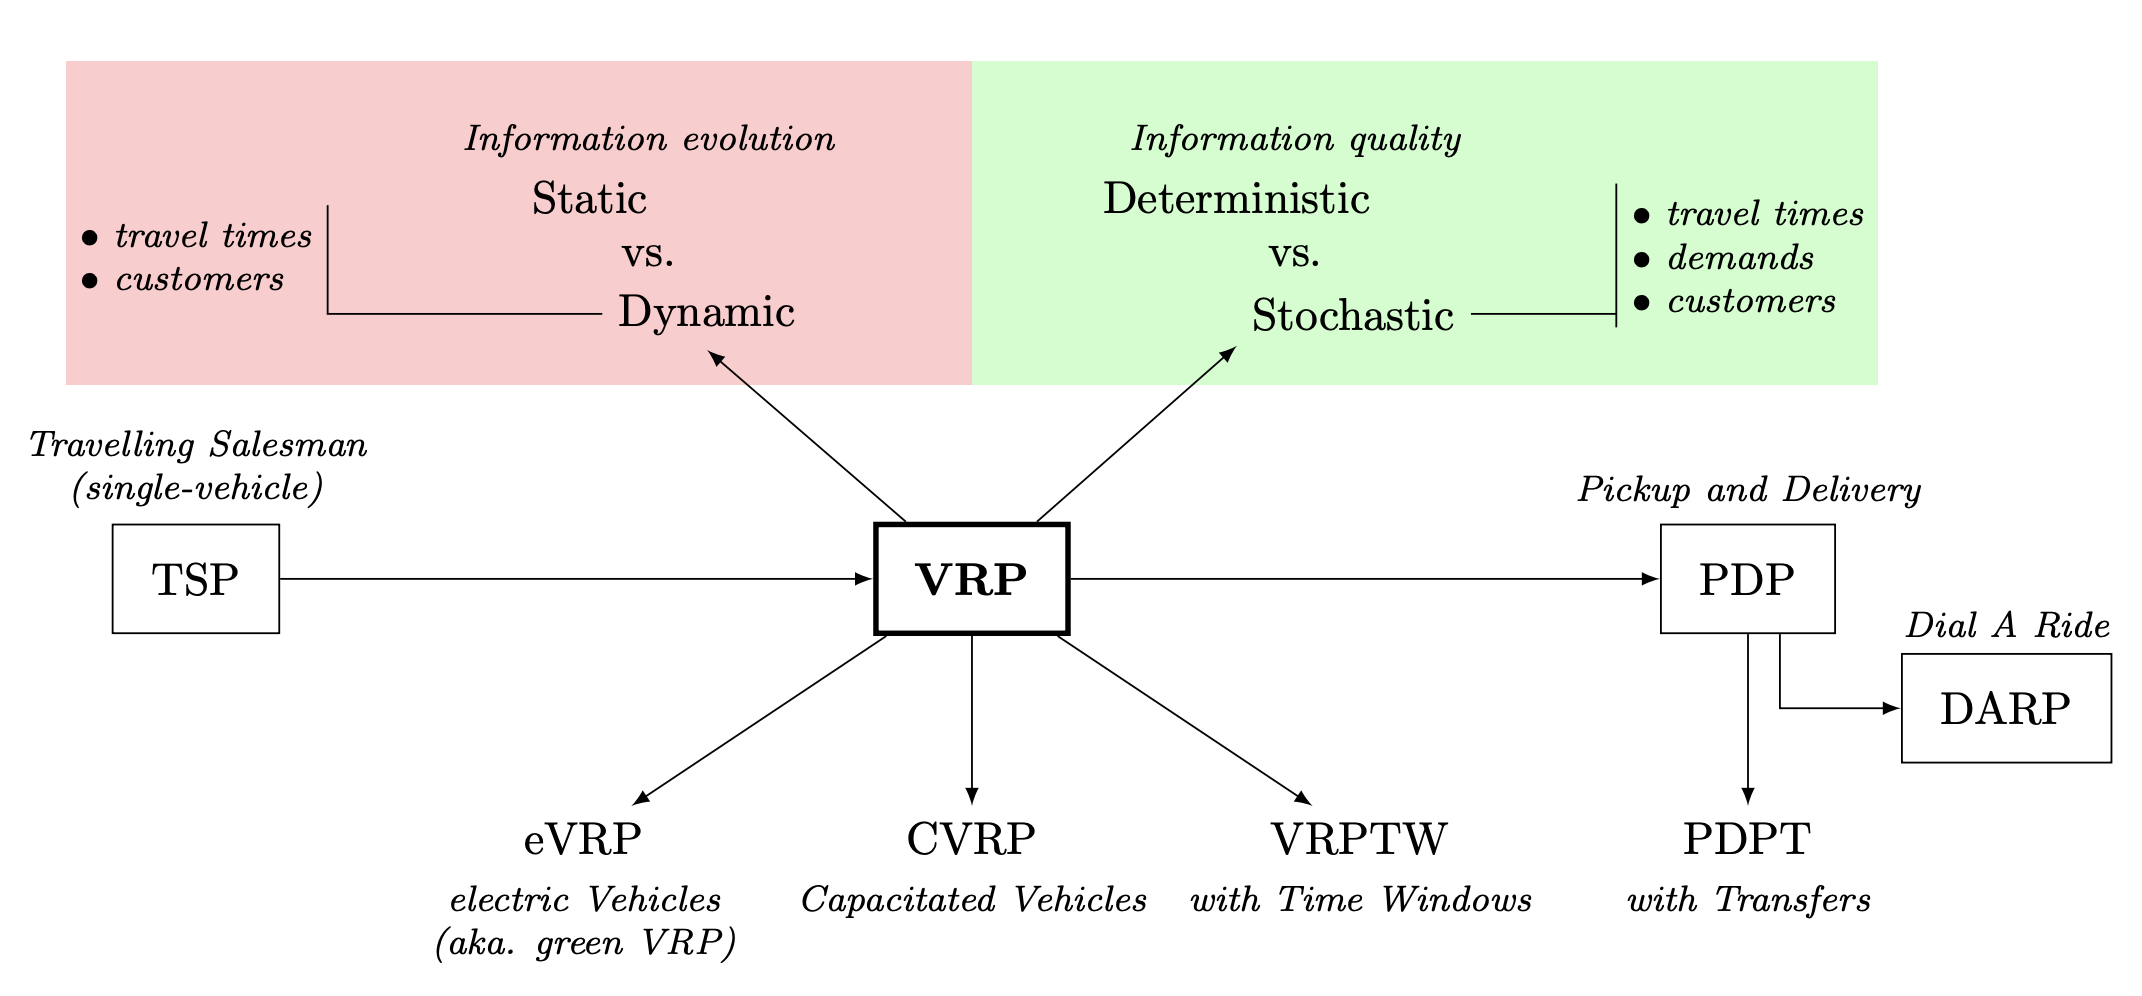
\includegraphics[width=1.0\textwidth]{resources/intro/vrp-flavours.png}
        \caption{Taxonomy of VRPs \cite{bono-stochastic-vrp}}
        \label{fig:vrp-flavours}
    \end{figure}

The sections below are describing each flavour shown in \ref{fig:vrp-flavours}.

    \subsection{Capacitated Vehicle Routing Problem}
    The \gls{cvrp} extends the regular \gls{cvrp} in introducing a capacity element for each customer. In the literature, it is sometimes referred to as a demand. The customer's demand is $d \in \mathbb{N}^+$ which may represent capacity in the form of weight, size but also in some abstract concepts such as a basket of apples. Additionally, each vehicle has a predefined capacity $Q > 0$.
    
    The \gls{cvrp} extends the solution feasibility formula by the following capacity constrain.
    \begin{equation}
        q(R) := \sum_{i \in R} d_i \leq Q
    \end{equation}
    
    If the vehicle capacity of the fleet stays the same, we are dealing with \gls{cvrp} with homogeneous fleet. A fleet with varying capacity for each vehicle is a heterogeneous fleet.
    
    \subsection{Vehicle Routing Problem with Time Windows}
    The \gls{vrptw} \cite{vrptw-solomon} extends the regular \gls{vrp} by time constraint for each customer. Customers have assigned time window interval $[e_i, l_i]$ where $e_li < l_i$. The time interval is the request within a vehicle is supposed to visit the node. 
    
    The time window can be either implemented as a hard constraint or a soft constraint. Hard constraint forces the vehicle to visit the node, i.e., the customer either in the given time interval or the solution is not feasible. Soft constrains are not strictly enforcing the vehicle to visit the customer, but they introduce a penalty for a violated interval barring a penalty cost. The penalty becomes a part of the cost function which \gls{vrp} aims to minimize.
    
    In this thesis, we will be focusing on soft constraints for time windows since it is a better reflection of real world use cases. Most businesses allow couriers to arrive late or early, but these types of arrivals are supposed to be minimized.
    
    \subsection{Pick and Deliver}\label{pick-and-delivery}
    The \gls{pdp} extends the regular \gls{vrp} by pairing pick and drop with precedence relationships, in which a pickup point must precede the paired delivery point. This flavour of \gls{vrp} is one of the most complex and even challenging for conventional methods like optimization heuristics algorithms.
    
    The feasibility of a \gls{pdp} solution is checking whether all delivery points have preceded pickup point.
    
    \subsection{Static vs. Dynamic}\label{dynamic}
    When solving the vehicle routing model, usually we assume that all the input data are static and known with certainty. However, this is not the case in real-life applications where data such as customer demand or travel time are often incomplete or not precise during the planning phase, they are only gradually revealed and specified.
    
    \textbf{Static \gls{vrp}} does not assume that the input data could be subject to change. The \textbf{dynamic \gls{vrp}} is aware about the information evolution\cite{psaraftis} and its goal is to obtain a robust routing planner that will be able to solve already seen instances with subject to small changes without the need of recalculating the whole instance again. This is called a priori optimization, after solving a given instance of a combinatorial optimization problem, it becomes necessary to repeatedly solve many other instances with a small variation from the original instance but without reconsideration of the entire problem \cite{apriori-optimization}.
    
    In this thesis, the \gls{vrp} based on \gls{ai} could be a great candidate for dynamic \gls{vrp} even though, the entire instance is being recalculated. The reason is that the problem solution is calculated in a seconds instead of minutes and the \gls{ai} technically already seen the instance in some variation during the training phase.
    
    Dynamic \gls{vrp} can be achieved with enough robust architecture around the core planner and periodically recalculating the instance with newly revealed information. The planner needs to take its previous solution as an input so the part of the problem does not need to be recalculated. This approach tends to be more exploitative since it is finding a solution in a predefined search space. It would benefit from introducing an explorative element which would diversify the search and could find better cost in a different local optimum.

    \subsection{Deterministic vs. Stochastic}\label{dynamic}
    Psaraftis \cite{psaraftis} stated that there are two important dimensions of input data, the information evolution which is used in dynamic \gls{vrp} and quality of information for stochastic \gls{vrp}. The majority of studied \gls{vrp} models are under the assumption that all the information necessary to formulate the problems is known and readily available. This is true but only for the deterministic settings \cite{vrp-bible}.
    
    A \textbf{\gls{vrp} is stochastic} \cite{stochastic-vrp} when some of its data behave as random variables, and the routes must be defined before the values of these random variables become known. Based on the probability distribution of the random variables, we may extract some hidden information and use it to our advantage in the planning process. The newly created plans will have incorporated stochastic information and the routing decisions may lead to different decisions because of the stochastic information being part of the cost function.
    
    A specific real-life example of stochastic \gls{vrp} would be if we consider an electric fleet of shared mobility vehicles and treat the locations of Blinkee electric scooters as random variables. Based on the probability distribution of Blinkee scooter, we may predict the time and location where a courier will transfer to a new fully charged Blinkee scooter. This action will be incorporated into the planned routes.
    
    In contrast, \textbf{deterministic \gls{vrp}} has no random information which could be leveraged before the execution of routes and all the given information are known with certainty. In this thesis, we are focusing on deterministic \gls{vrp}.
    
    \subsection{Other Flavours}
    Dial-a-Ride (DARP) proposed by Wilson et al. \cite{darp-proposed} in 1971 is a special case of dynamic \gls{vrp} with pick and deliver. Passengers request a ride at a specified origin and drop location with an optional time window. 
    
    \label{split-delivery}Split Delivery \gls{vrp} \cite{split-deliver} is a variant where customers are allowed to be visited more than once. This can be convenient for deliveries of large capacity or stocking fulfillment centers.
    
    Multi Depot \gls{vrp} is a simplification of the vehicle routing problem with pick and deliver, where pick can happen only on predefined depot locations. This simplification of pickup location is making the problems less complex then \gls{vrppd}.
    
\section{VRP in a Real-world}
Consumer habits have been shifting towards online and the pandemic situation only accelerated this process. Delivery option is nowadays taken for granted and consumers are demanding a perfect delivery experience. In 2020, there has been shipped over 5.5 billion packages around the world \cite{num-shipped-packages}.

Solving various flavors of \gls{vrp} efficiently in a reasonable time plays a crucial role for multiple businesses. For example, urban logistics is an essential part of the delivery process, not only it is the last part of the delivery chain, but frequently the courier interacts with the customer and delivery on time with proper ETA prediction is a must. It is also the most expansive part which makes up about 53\% of shipment’s total cost\cite{num-shipped-packages}. Urban logistics by large benefits from a better and more optimized \gls{vrp} which increase the delivery efficiency and reduces the delivery cost.

\begin{figure}[ht]
    \centering
    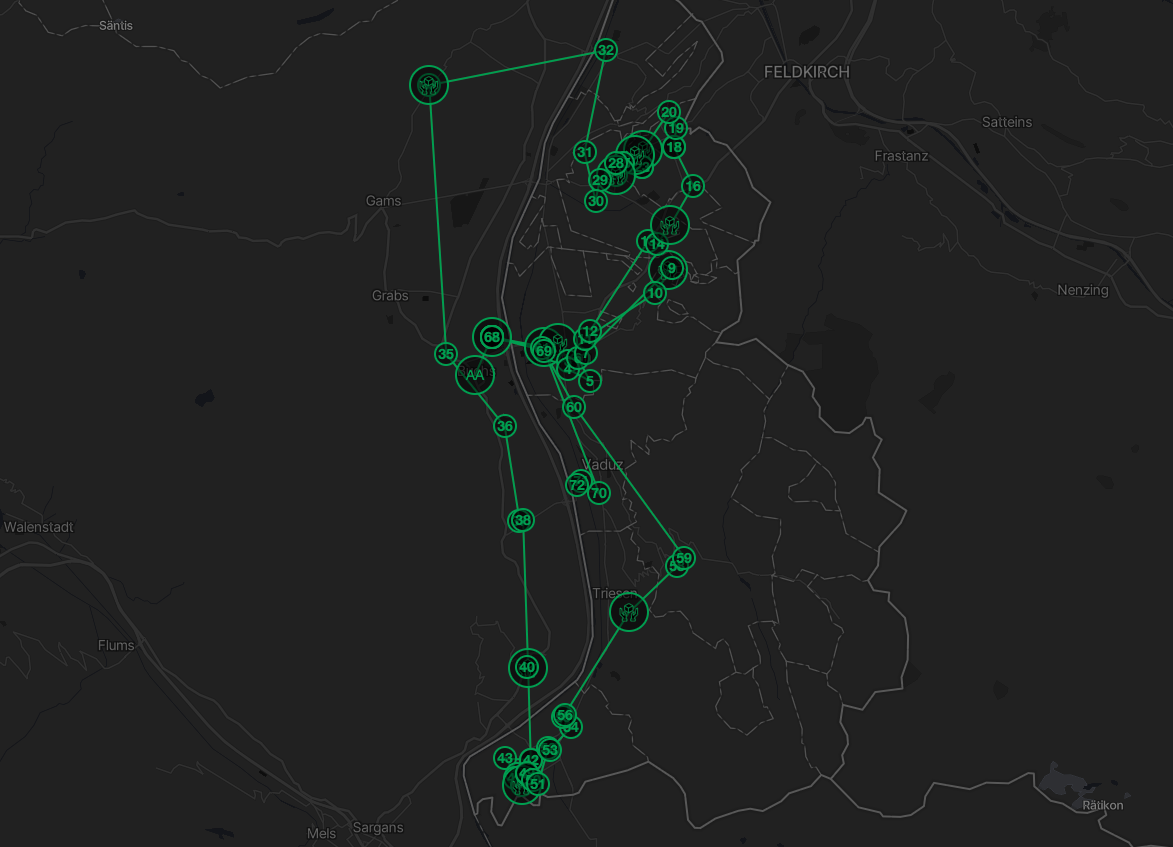
\includegraphics[width=0.75\textwidth]{resources/intro/hofkorb.png}
    \caption{Grocery delivery planning with multiple depots from the GoDeliver system}
    \label{fig:hofkorb}
\end{figure}

At GoDeliver, we are building an autonomous last-mile delivery system and at the core is a planning system which is solving various \gls{vrp}. The flavour which we are focusing on is Dynamic Capacitated Vehicle Routing Problem with Time Windows and Pick and Delivery (CVRPDPTW). GoDeliver typical use case is on-demand food delivery with multiple depots (pick and deliver), this means that the system has to be dynamic and flexible because a new customers are ordering stochastically for a chosen time window. Another our common use case shown in \ref{fig:hofkorb} is grocery delivery with multiple depots, time windows, and capacity for customers.

    \chapter{Theoretical Background}\label{theoretical_background}

In this chapter, we will be covering the advanced theoretical background to fully understand the solved task of \gls{vrptw} using \gls{ai}.

\section{Reinforcement Learning}\label{rl}
    \gls{ml} can be divided with a little simplification into three categories; supervised learning, unsupervised learning, and reinforcement learning. Supervised learning is the most common where the model is learned from the provided labeled data. Unsupervised learning, on the other hand, is about finding a hidden patterns in a collection of data with no labels. Finally, reinforcement learning has no labeled data but learns by interacting with the environment and getting feedback in the form of rewards as shown in Figure \ref{fig:rl-loop}. 
    
    \begin{figure}[ht]
        \centering
        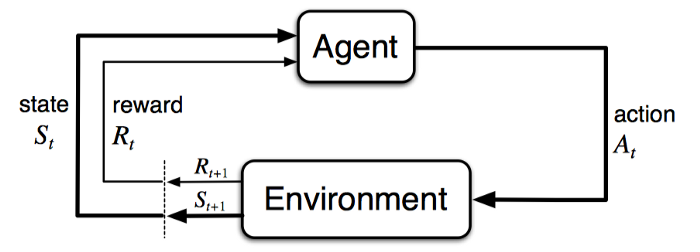
\includegraphics[width=0.75\textwidth]{resources/theoretical-background/rl-loop.png}
        \caption{Agent feedback loop\cite{rl-intro}}
        \label{fig:rl-loop}
    \end{figure}
    
    The Reinforcement Learning mimics the learning process of humans beings. By experiencing the world and accumulating knowledge, we are learning how to handle novel situations. \gls{rl} system consists of agent in observed state $s_t$, the agent interacts with the environment via its actions $a_t$ at discrete time steps $t$ and receives a reward $r_{t+1}$ for given action. The action moves the agent into a new state $s_{t+1}$. The goal of the agent is to learn a policy $\pi$ which chooses the action that maximizes the agent's rewards based on the environment \cite{rl-intro}. 
    
    %The policy is formally defined as a probability distribution of 
    \subsection{State and Action Value Functions}
        Transition to a new state gives us a reward and to maximize it, we need a way to quantify how good a state is. A state-value function $V_{\pi}(s)$ predicts a future reward for a given state when following the policy $\pi$ \cite{rl-intro}. 
    
        \begin{equation}
            V_{\pi}(s) = \mathop{\mathbb{E}}[G_t|S_t = s]
        \end{equation}
        \begin{equation}\label{discount-reward}
            G_t = \sum_{k=0}^{\infty} \gamma^k R_{t+k+1}
        \end{equation}
        The equation \ref{discount-reward} calculates $G_t$, all future rewards, sometimes called as $return$ \cite{rl-intro}. The $\gamma \in [0,1]$is a discount factor and penalizes the rewards in the future, incorporating the possible uncertainty and variance of the future rewards.
    
        We will also define action-value $Q_{\pi}(s, a)$ which is for a similar purpose as state-value function but predicts the reward for action and state following the policy $\pi$.
        \begin{equation}
            Q_{\pi}(s, a) = \mathop{\mathbb{E}}[G_t|S_t = s, A_t = a]
        \end{equation}
        
        The decomposition of state-value and action-value function replays on Bellman equations \cite{bellman-eq}. The decomposition of state-value function is
        \begin{equation}
            V_{\pi}(s) = \mathop{\mathbb{E}}[G_t|S_t = s]
        \end{equation}
        \begin{equation}
            V_{\pi}(s) = \mathop{\mathbb{E}}[R_{t+1} + \gamma R_{t+2} + \gamma^2 R_{t+3} + \cdots |S_t = s]
        \end{equation}
        \begin{equation}
            V_{\pi}(s) = \mathop{\mathbb{E}}[R_{t+1} + \gamma(R_{t+2} + \gamma R_{t+3} + \cdots) |S_t = s]
        \end{equation}
        \begin{equation}
            V_{\pi}(s) = \mathop{\mathbb{E}}[R_{t+1} + \gamma G_{t+1} |S_t = s]
        \end{equation}
        \begin{equation}
            V_{\pi}(s) = \mathop{\mathbb{E}}[R_{t+1} + \gamma V(S_{t+1}) |S_t = s]
        \end{equation}
        Similarly, this method is applicable to action-value function,
        \begin{equation}
            Q_{\pi}(s, a) = \mathop{\mathbb{E}}[R_{t+1} + \gamma V(S_{t+1}) |S_t = s, A_t = a]
        \end{equation}
        \begin{equation}
            Q_{\pi}(s, a) = \mathop{\mathbb{E}}[R_{t+1} + \gamma \mathop{\mathbb{E}}_{a \sim \pi} Q(S_{t+1}, a) |S_t = s, A_t = a]
        \end{equation}
    
        \subsection{Policy Gradients}
        Policy Gradient \cite{policy-gradient} is a method for solving the reinforcement learning problem and learning the policy that maximizes the rewards. We define a set of parameters $\theta$ that directly models the policy, $\pi_{\theta}(a|s)$.
    
        To optimize $\theta$ for the best reward, we define an objective function \cite{policy-gradient} as
        \begin{equation}
            J(\theta) = \sum_{s \in S} d_{\pi_{\theta}}(s)V_{\pi_{\theta}}(s)
        \end{equation}
        where $d_{\pi_{\theta}}(s)$ is stationary distribution of Markov chain for $\pi_{\theta}$, the probability of ending in a given state \cite{markov-bullshit}.
        \begin{equation}
            d_{\pi_{\theta}} = \lim_{t -> \infty} P(S_t = s | s_0, \pi_{\theta})
        \end{equation}
        
        The objective function $J(\theta)$ optimizes the $\theta$ parameters via gradient ascent [TODO]. 
        \begin{equation}
            \theta_{t+1} = \theta_{t} + \alpha \nabla J(\theta_{t})
        \end{equation}
        However, computing $\nabla J(\theta)$ is tricky because it depends on the action selection and the stationary distribution of states \cite{policy-weng}. Policy gradient can be simplified using Policy Gradient Theorem by Sutton et al. \cite{policy-gradient}.
        
        The proof of policy gradient theorem is quite long and complicated, but you may go through it in this article \cite{policy-weng} which is inspired by Sutton and Barto \cite{rl-intro}. Policy gradient is simplified to the form as
        \begin{equation}
            \nabla J(\theta) = \mathop{\mathbb{E}}[ \nabla \ln \pi (a|s, \theta) Q_{\theta}(s, a)]
        \end{equation}
    
        \subsection{REINFORCE}\label{reinforce}
        REINFORCE algorithm proposed by Williams \cite{reinforce} in 1992 is a policy gradient method to update the policy parameter $\theta$.
        
        \begin{algorithm}
        \end{algorithm}
    

    \section{Attention Mechanism}\label{attention}
    TODO    

    \subsection{Transformer}\label{transformer}
    TODO
    
    \subsection{Graph Attention Network}\label{graph-attention-network}
    TODO
    
    


    
    % bibliography
    \bibliographystyle{prefs/iso690}
    \bibliography{ref}
    
    \appendix
    
    % acronyms
    \printglossaries
    
    % media contents
    \chapter{Media contents}\label{app:CDcontent}
    \begin{figure}
    	\dirtree{%
    		.1 readme.txt\DTcomment{the file with CD contents description}.
    		.1 data\DTcomment{the data files directory}.
    		.2 example\textunderscore sequence\DTcomment{the directory with example sequence from dataset}.
    		.3 *.jpg\DTcomment{the example images}.
    		.2 example\textunderscore sequence\textunderscore graphs\DTcomment{the directory of graphs of experiments}.
    		.3 *.png\DTcomment{the motion output graphs}.
    		.2 tracking\textunderscore example.mp4\DTcomment{the example video file}.
    		.1 src\DTcomment{the directory of source codes}.
    		.2 models\DTcomment{the directory of deep learning modules}.
    		.2 utils\DTcomment{the directory of helper modules}.
    		.2 *.py\DTcomment{the Python source files}.
    		.1 text\DTcomment{the thesis text directory}.
    		.2 thesis\DTcomment{the directory of \LaTeX{} source codes of the thesis}.
    		.2 thesis.pdf\DTcomment{the Diploma thesis in PDF format}.
    	}
    \end{figure}
    

\end{document}
